\section{Wetting and drying}
\label{sec:wd}

Tests 4.5 and 4.7 of \citet{ma2012} and the surf-zone example of the NHWAVE
repository need moving shorelines. This section describes the wetting and
drying of \NHFOAM, which follows NHWAVE's mask and thin film
\citep[][Section~3.4]{ma2012} but had to be adapted to the implicit free
surface and the collocated mesh, compares the two treatments, and tests them:
still water against a dry beach, the oscillation in a parabolic basin of
\citet{thacker1981} and a dam break on a dry bed (verification), and the
run-up of a breaking solitary wave \citep{synolakis1987}, the solitary waves
on a conical island of \citet{briggs1995}, the tsunami run-up in the Monai
valley \citep{matsuyama2001}, also on meshes refined around the valley, and
the spilling breakers of \citet{ting1994} (validation, with NHWAVE).

\subsection{Method}
\label{sec:wd-method}

\paragraph{Mask.} A dry column keeps a film of depth $D_{\min}$
(\code{minDepth}), so $\eta = z_b + D_{\min}$. The mask is updated at the start
of every time step from $\eta^n$, with NHWAVE's rules: a dry column floods when
a wet neighbour has a higher surface and more than the film,
$\eta_w > \eta_d$ and $D_w - D_{\min} > \epsilon$; a wet column dries when
$D - D_{\min} \le \epsilon$ ($\epsilon = 10^{-6}$ m), and its surface is then
reset to the film. A column that changes state starts from the film at both
stored time levels, so the BDF2 time derivative sees no jump. A side face is
open when the columns on both sides are wet. A closed face carries no flux and
has no coefficients in the pressure matrix, and in the cell-centred pressure
gradient it acts as a wall: each side sees its own pressure, so a dry
neighbour exerts no force and still water stays at rest against a dry beach.
The velocity of dry columns is held at zero by an implicit sink,
$10^4/\Delta t$ on the diagonal of the momentum equation. The same is done in
a wet column whose side faces are all closed (a puddle left on the beach): its
velocity could only carry it away from the lower neighbour it floods next.

\paragraph{Positivity.} The implicit pressure solve can draw more water from
a shallow column than it holds. After the solve, the side outflows of a column
are limited so that its surface stays at or above the film at the new level:
with the free-surface update of \eqref{eq:bdf2}, the net side outflow may not
exceed
\begin{equation}
  Q_{\max} = -\phi_{\mathrm{bottom}} - \frac{A_h}{a}\left(\eta_{\min} - \hat\eta\right),
  \qquad \eta_{\min} = z_b + D_{\min},
\end{equation}
(relaxation-zone terms included in the code). The outflows of a column that
would exceed it are scaled down by a common factor; this lowers the inflow of
its neighbours, so the sweep is repeated until no column exceeds its limit.
Inflows are never changed by a column's own limit and each face keeps one
value, so volume is conserved to round-off. The only loss is the reset of a
drying column, at most $\epsilon$ per column.

\paragraph{Water depth at the side faces.} The mesh face between two columns
has the depth of the vertical point lines at the column edge, about the mean
of the two columns. With this centred depth the first version of the method
moved flood fronts too slowly and let bores in thin water oscillate: a dam
break on a dry bed advanced at 0.9 m/s where NHWAVE gives 1.25 m/s
(Section~\ref{sec:wd-dambreak}), and the solitary wave of
Section~\ref{sec:wd-runup} ran up to $R/d = 0.41$ instead of 0.51. As in the
semi-implicit schemes of \citet{stelling2003b} and SWASH, the side fluxes now
carry the water depth on the upwind side,
\begin{equation}
  D_f = \eta_f - z_{b,f},\qquad
  \eta_f = \eta_C + \tfrac12\,\psi(r)\,(\eta_D - \eta_C),\qquad
  r = \frac{2\,\bm{d}\cdot\nabla\eta_C}{\eta_D - \eta_C} - 1,
  \label{eq:facedepth}
\end{equation}
where $C$ is the upwind and $D$ the downwind column, $\bm{d}$ the vector
between their centres, $z_{b,f}$ the bottom of the face and $\psi$ a TVD
limiter (van Leer by default; minmod, MC, or $\psi=0$ for the first-order
upwind depth, can be chosen). Next to a column with less than two films of
water the surface ends, and the upwind value is used. All layer fluxes of the
face are scaled by $f = D_f/D_{\mathrm{mesh}}$: in the predicted flux
$\phi_{\mathrm{HbyA}}$, in the implicit coefficients of the pressure matrix and
in the convecting flux of the momentum equation. The face velocity
$\bm{u}_f$, which carries the flux of a time step to the next one (the
$\partial\bm{u}/\partial t$ flux correction and the flux extrapolation of
Section~\ref{sec:time}), stays the flux divided by $f$, so it is not scaled
twice. NHWAVE gets the same upwinding from its MUSCL reconstruction and HLL
fluxes.

\paragraph{Supercritical faces.} Where the upwind column is supercritical,
with a depth-averaged velocity normal to the face above
$\mathrm{Fr}_c\sqrt{gD}$ (\code{upwindFroude}, default 1), the predicted flux of
the face is that of the upwind cell, $\bm{H}_C\cdot\bm{S}_f$, instead of the
interpolated one. An HLL flux does the same once both wave speeds have the
sign of the flow. Without it, the face at the tip of a run-up carries the mean
of a fast and a slow (or resting) column. The switch must stay sharp. When the
upwind flux was blended in below $\mathrm{Fr} = 1$, grid-scale oscillations
grew in the subcritical part of a dam break: the interpolated flux is what
couples pressure and velocity on the collocated mesh, and upwinding it at all
faces next to shallow water made the solution noisy everywhere. A blend
between $\mathrm{Fr} = 1$ and 1.5 lowered the run-up by 10\%.

\paragraph{Faces opened by flooding.} In the step after a column floods, the
predicted flux of the faces it opened may only run into it, since its film
cannot feed the flow. Where it lies lower than the wet column, the face
velocity is at least that of a dam break from rest at the dam,
$\tfrac23\sqrt{g(D_w - D_{\min})}$. Without these two rules a puddle flooded its
lower neighbour every other step without water flowing into it (the flux was
cut to zero by the positivity limiter, and the neighbour dried again); applied
up the slope as well, the dam-break velocity made a film creep up the whole
beach.

\paragraph{Options.} \code{hydrostaticDepth} switches the non-hydrostatic
pressure off in columns shallower than the given depth (as the breaking
columns of Section~\ref{sec:numhfa}). \code{bottomFriction} adds the quadratic
stress $\bm{\tau}_b/\rho = C_d\,|\bm{u}_b|\,\bm{u}_b$ on the bottom cells,
with a constant $C_d$ or $C_d = g n^2/D^{1/3}$ from a Manning coefficient $n$
(it can be used without wetting and drying). The wetting and drying needs the
interface pressure layout. The highest wet bed and the highest surface on land
are written every step to \code{postProcessing/wettingDrying}.

\paragraph{Nonlinear waves.} For the surf-zone test the relaxation zones were
given a second target, the stream-function wave of \citet{fenton1988}: a
Fourier series of order $N$ for $\eta$ and for the stream function, whose
coefficients are computed beforehand (\code{validation/stream\_function.py},
zero mass flux by default, i.e.\ with the return current of a closed flume).
In a flat flume, $h = 0.4$ m, 10 layers and $\Delta x = 2.5$ cm, the zone made
the wave of \citet{ting1994} ($H = 0.125$ m, $T = 2$ s, Ursell number 27)
with $H = 0.1246$--$0.1249$ m at six gauges over 10 m, crest and trough
within 1.4 and 1.1 mm of the theory, and no beating of free harmonics.

\subsection{Comparison with NHWAVE}
\label{sec:wd-nhwave}

Table~\ref{tab:wd-features} sets the two treatments side by side; the NHWAVE
column is read from the source (\code{update\_mask}, \code{construction},
\code{flux\_bc} and \code{eval\_duvw} in \code{nhwave.F}). The mask and the
closed faces are the same. The differences come from the time integration.
NHWAVE updates the depth explicitly from Riemann fluxes, so positivity is a
clip and the upwinding of depth and velocity is built into the HLL flux.
\NHFOAM's surface is implicit, so the outflows must be limited after the
solve, and the upwinding has to be added to the depth and to the predicted
flux explicitly.

\begin{table}[ht]
\centering
\caption{Wetting and drying in NHWAVE and \NHFOAM.}
\label{tab:wd-features}
\small
\begin{tabular}{p{3.0cm}p{5.6cm}p{5.6cm}}
\toprule
 & NHWAVE & \NHFOAM \\
\midrule
mask & from $\eta^n$ at each step: flood if a wet neighbour is higher and has more than the film; dry at the film & same \\
dry cells & $D = D_{\min}$, not updated & $\eta = z_b+D_{\min}$, velocity held at zero \\
faces of dry cells & no mass flux; momentum flux is the wet side's hydrostatic pressure (a wall) & closed: no flux, a wall for the pressure gradient \\
positivity & $D = \max(D, D_{\min})$ after each stage (adds water) & limiter on the outflows (conservative) \\
depth at wet faces & MUSCL (van Leer) reconstruction of $\eta$, HLL flux & TVD (van Leer) reconstruction of $\eta$, upwind next to near-dry columns \\
supercritical faces & HLL takes the upwind flux & predicted flux of the upwind cell \\
newly wet faces & HLL depth diffusion, $\sim c\,\Delta D/2$ & flux only into the new column; dam-break velocity downhill \\
puddles & spread by the HLL diffusion & held at rest until they flood a lower neighbour \\
$q$ in thin water & solved everywhere, no correction in dry cells & solved everywhere; optional $q = 0$ below a depth \\
breaking & shock capturing ($k$--$\epsilon$ in the surf-zone example) & hydrostatic front approximation \\
volume & not conserved exactly (clip) & conserved; a drying column loses $\le\epsilon$ \\
\bottomrule
\end{tabular}
\end{table}

\subsection{Still water and the parabolic basin}
\label{sec:wd-thacker}

Still water against a dry 1:20 beach (film 5 mm, $\Delta x = 5$ cm, 3 layers)
stays at rest: after 10 s the largest velocity is $5\times10^{-9}$ m/s and the
surface deviates by $3\times10^{-10}$ m.

In the parabolic basin $z_b = h_0\,[(x-L/2)^2/a^2 - 1]$ of \citet{thacker1981},
the surface stays planar and oscillates with the period
$T = 2\pi a/\sqrt{2gh_0}$, and both shorelines move by $\pm a\beta$, with
$\beta = B/(a\omega)$. With $a = 100$ m, $h_0 = 0.5$ m, $B = 0.5$ m/s
($T = 200.6$ s), the basin was approximated by 80 straight segments, with
$\Delta x = 1$ m, 3 layers, $\Delta t = 0.25$ s and a 1 mm film
(Fig.~\ref{fig:wd-thacker}). Over two periods the rms error of the surface is
0.3--1.5 mm (0.9 mm overall) and the largest error 7.4 mm, for a surface that
moves by $\pm0.16$ m at the shorelines. The shorelines, taken as the centre of
the last wet column, are within 1.7 m of the exact ones (0.8 m on average, for
$\Delta x = 1$ m), with no drift from the first to the second period.

\begin{figure}[ht]
\centering
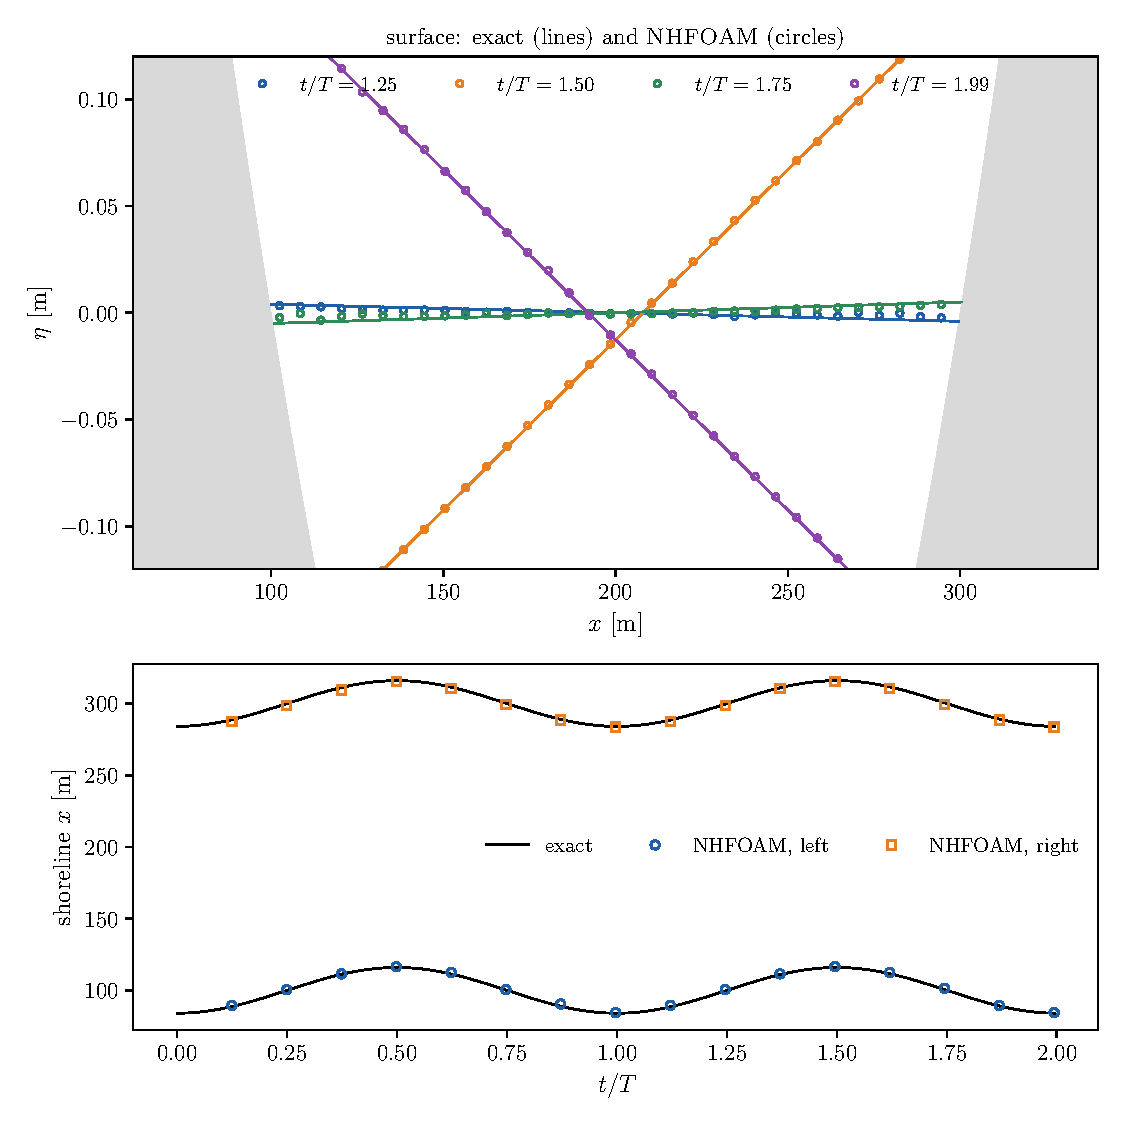
\includegraphics[width=0.85\textwidth]{wd_thacker.pdf}
\caption{Parabolic basin of \citet{thacker1981}: surface at four times of the
second period and the two shorelines over two periods.}
\label{fig:wd-thacker}
\end{figure}

A narrow cell at the shoreline is a hard case. In an earlier mesh, the point
where the depth equals the film was a block vertex, which left a column of
0.1 m among columns of 1 m. With the TVD depth, that column kept a puddle,
because its gradient, taken from its one open face, made the reconstruction
of \eqref{eq:facedepth} reach the dry downwind level. The upwind depth next to
near-dry columns removed the puddle. The errors on that mesh are still four
times larger (rms 3 mm), and the validation meshes avoid such cells.

\subsection{Dam break on a dry bed}
\label{sec:wd-dambreak}

Water of depth $h_0 = 0.1$ m is released at $x = 5$ m onto a dry, flat,
frictionless bed ($\Delta x = 2$ cm, 3 layers, $\Delta t = 4$ ms, film 1 mm,
hydrostatic). \citet{ritter1892}'s solution has a front that runs at
$2\sqrt{gh_0} = 1.98$ m/s with vanishing depth. Neither model gets near it
(Fig.~\ref{fig:wd-dambreak}): both treat the film of the dry columns as water
at rest, which the flow has to push, and both follow the solution of
\citet{stoker1957} for a wet bed as deep as the film, a bore of 1.7 cm moving
at 1.23 m/s. The fronts at $t = 1$, 2 and 3 s are at 6.21, 7.59 and 8.95 m in
\NHFOAM, 6.27, 7.53 and 8.77 m in NHWAVE (MinDep 1 mm) and 6.23, 7.47 and
8.70 m in Stoker's solution. With the centred face depth the front of
\NHFOAM\ moved at 0.9 m/s, behind a pile-up of water at the tip. The film
therefore sets a lower limit to the depth of the flows that a run-up
computation can resolve: with a 5 mm film, as in the next test, a swash
lens of 2--3 cm is a bore over a bed that is a fifth of its depth.

\begin{figure}[ht]
\centering
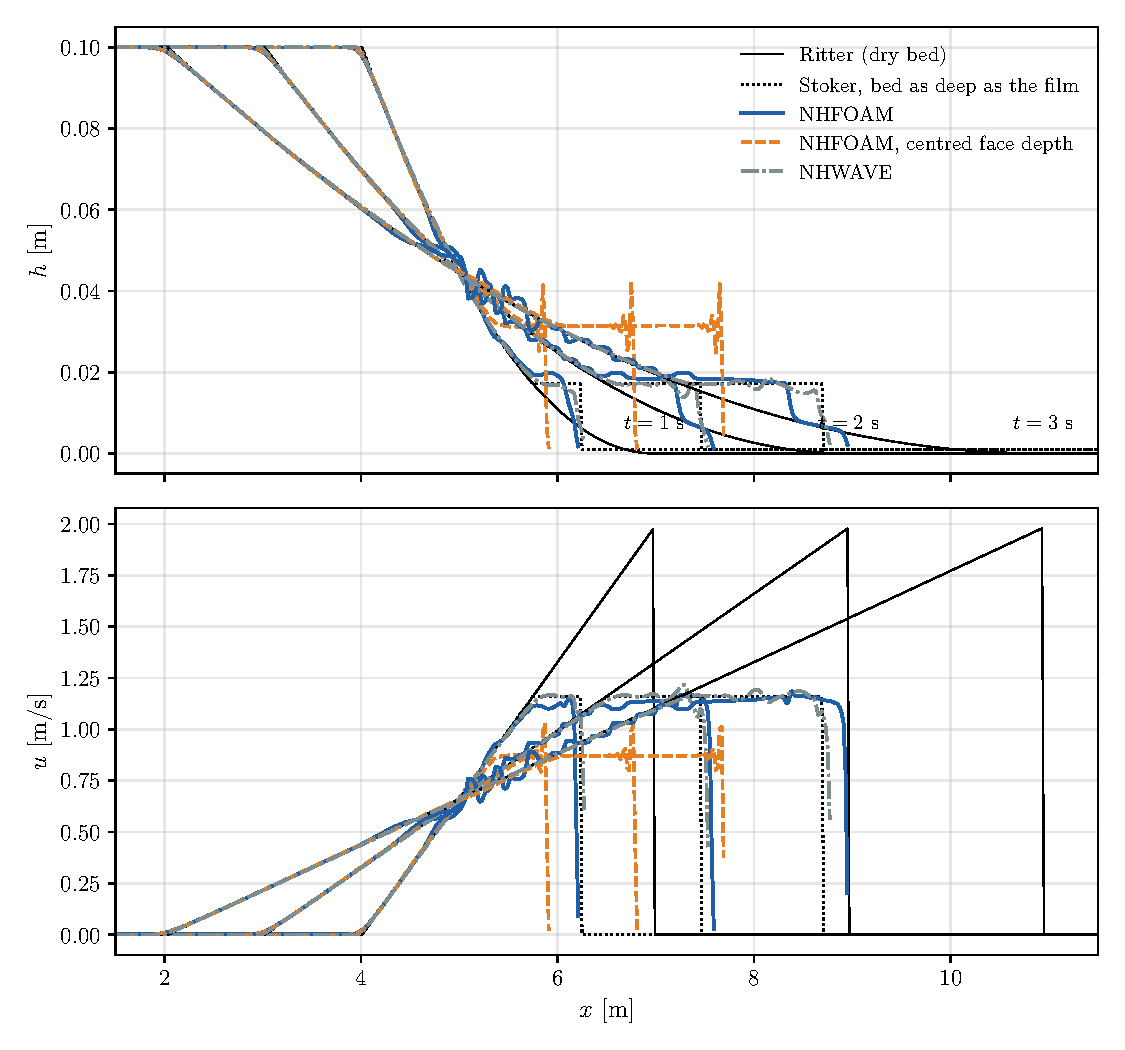
\includegraphics[width=0.85\textwidth]{wd_dambreak.pdf}
\caption{Dam break on a dry bed: depth and velocity at $t = 1$, 2 and 3 s.}
\label{fig:wd-dambreak}
\end{figure}

\subsection{Breaking solitary wave on a beach (test 4.5 of Ma et al.)}
\label{sec:wd-runup}

A solitary wave of $H/d = 0.28$ in $d = 0.21$ m breaks on a 1:20 beach
\citep{synolakis1987}, benchmark 4 of the NTHMP \citep{synolakis2008}, whose
data give the measured profiles. The set-up is NHWAVE's example
\code{solitary\_wave\_breaking}: toe at $x = 4$ m, the still-water shoreline at
8.2 m, dry beach up to 11 m, $\Delta x = 2$ cm, 3 layers, a 5 mm film. Both
models start from the solitary wave with its crest $d\,\mathrm{acosh}(\sqrt{20})/\gamma$
offshore of the toe ($\gamma = \sqrt{3H/4d}$), from the exact solution of
\citet{babenko1987} rather than NHWAVE's boundary wavemaker. NHWAVE's example
runs without bottom friction (no viscous terms, free-slip bottom), and so does
\NHFOAM\ here. \NHFOAM\ uses the hydrostatic front approximation and
\code{limitedLinearV}, with $\Delta t = 2$ ms.

The profiles (Fig.~\ref{fig:wd-runup}) agree with the measurements and with
NHWAVE during shoaling ($t^* = t\sqrt{g/d} = 10$, 15). At breaking ($t^*=20$)
\NHFOAM's bore is 0.04$d$ higher than NHWAVE's and the measured one. The
uprush ($t^* = 25$, 30) and the backwash with its hydraulic jump at
$x \approx 2.3d$ ($t^* = 50$) follow NHWAVE closely. The maximum run-up
(Fig.~\ref{fig:wd-shoreline}) is $R/d = 0.531$ at $t^* = 42.5$, against 0.512
at $t^* = 44$ for NHWAVE and 0.487--0.551 in the experiments with
$H/d = 0.26$--0.30. With the first-order upwind depth it is the same, 0.531;
with the centred depth 0.41; with $C_d = 0.006$ it is 0.464. In the backwash
the highest wet column of \NHFOAM\ recedes more slowly than NHWAVE's, because
thin puddles of up to a few millimetres above the film remain on the upper
beach. NHWAVE spreads such remnants with the depth diffusion of its HLL flux,
and its clip to the film does not conserve volume.

\begin{figure}[ht]
\centering
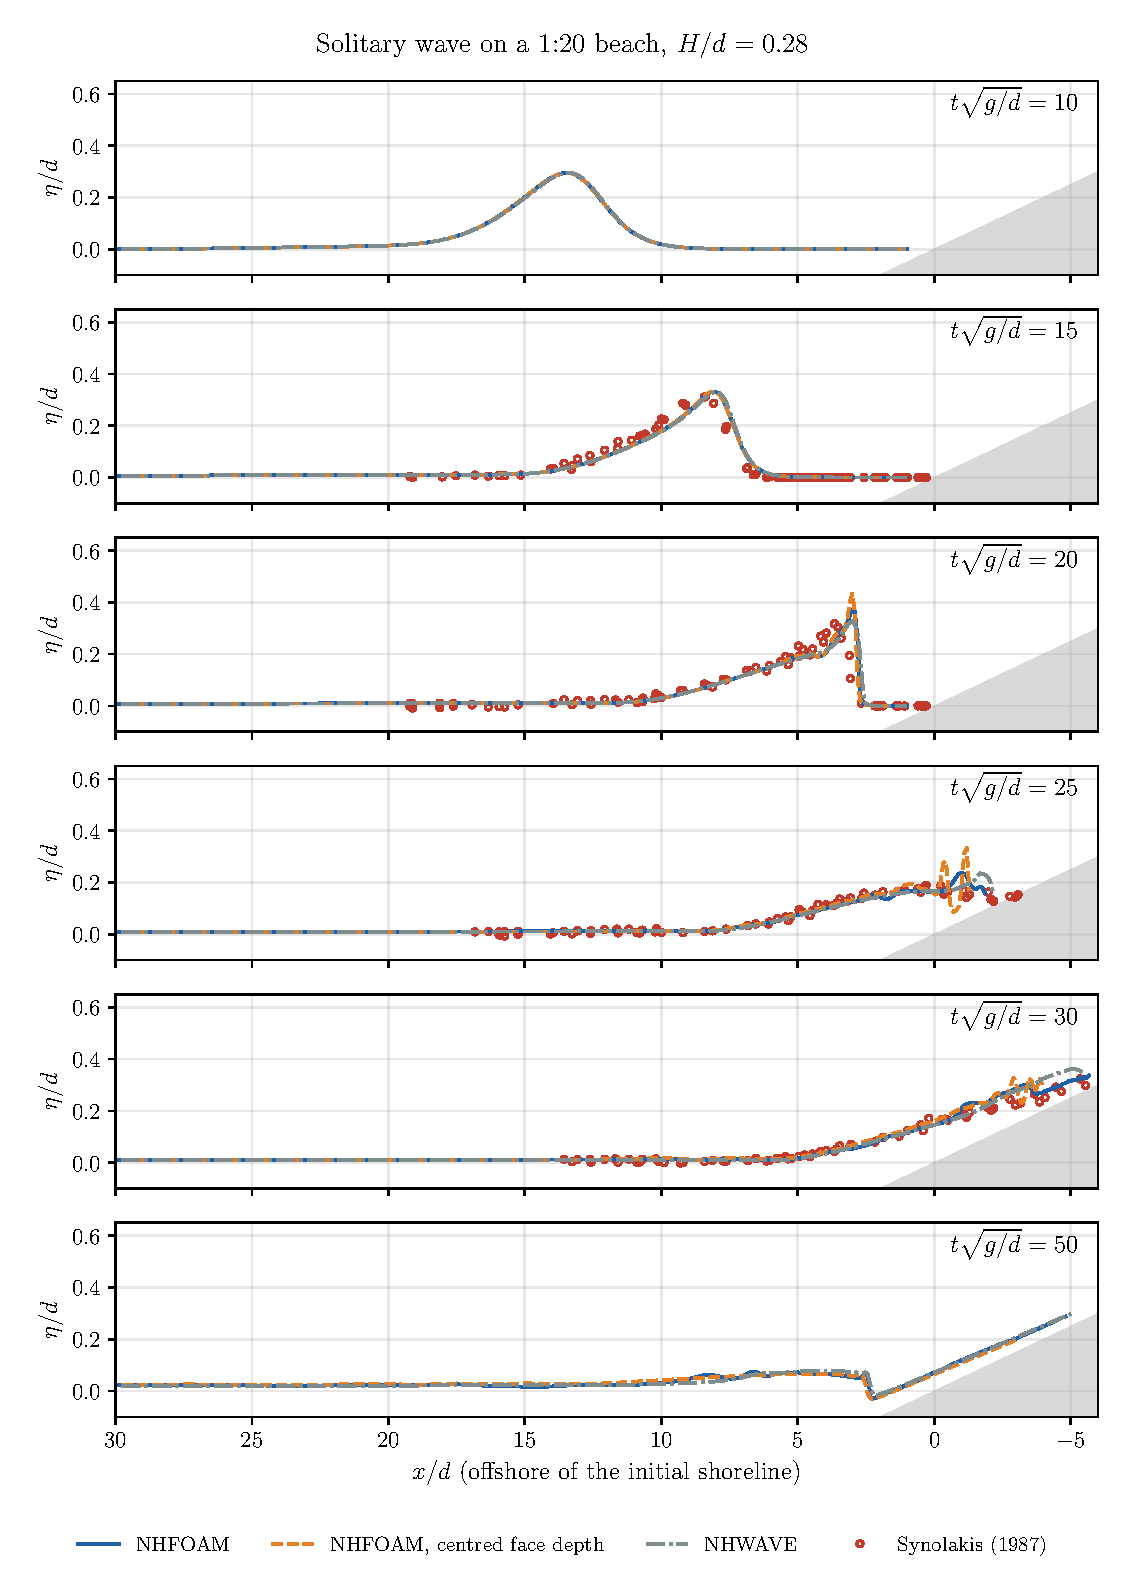
\includegraphics[width=0.88\textwidth]{wd_runup.pdf}
\caption{Solitary wave on a 1:20 beach, $H/d = 0.28$: surface profiles against
the measurements \citep{synolakis1987}.}
\label{fig:wd-runup}
\end{figure}

\begin{figure}[ht]
\centering
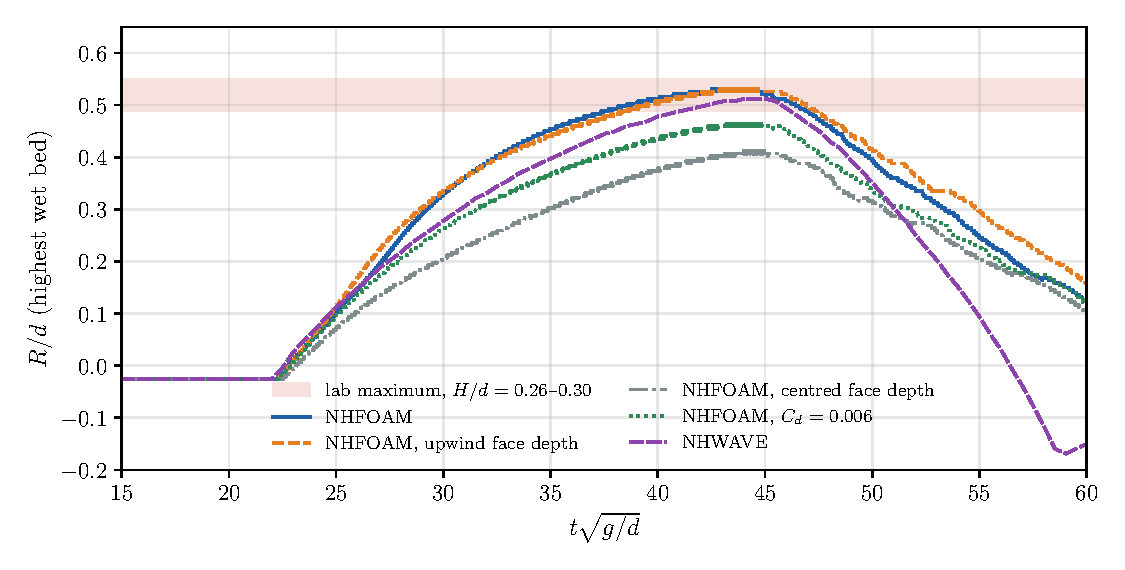
\includegraphics[width=0.9\textwidth]{wd_runup_shoreline.pdf}
\caption{Solitary wave on a 1:20 beach: highest wet bed over time. The band
is the range of the measured maximum run-up for $H/d = 0.26$--0.30.}
\label{fig:wd-shoreline}
\end{figure}

The first versions of the method failed this test in instructive ways. With
the centred depth and newly flooded columns starting from rest, the run-up was
$R/d = 0.37$--0.41, and the swash had grid-scale oscillations of the depth:
columns of 5 mm between columns of 5 cm, flooding and drying every step.
Giving a flooded column the velocity of the neighbour that flooded it
overshot to $R/d = 0.66$: a film with that velocity floods the next column in
the next step, and it ran away to the end of the beach. The upwind face
depth, the supercritical flux and the rules for opened faces and puddles
removed both problems.

\subsection{Solitary waves on a conical island}
\label{sec:wd-island}

\citet{briggs1995} sent solitary waves of $H/d = 0.045$, 0.091 and 0.181
(cases A, B, C; $d = 0.32$ m) against a conical island with a toe radius of
3.6 m, a crest radius of 1.1 m and 1:4 faces, and recorded the water level in
front of the island (gauges 1--4), on its front face (6, 9), on its side (16)
and behind it (22), and the run-up all round \citep[see also][]{liu1995}. It
is benchmark 6 of the NTHMP \citep{synolakis2008}, one of NHWAVE's examples
(\code{Solitary\_wave\_on\_a\_conical\_island}) and the first test of wetting
and drying in three dimensions here.

Both models use the settings of NHWAVE's example: 3 layers, $C_d = 0.01$, a
5 mm film, NHWAVE with its $k$--$\varepsilon$ model and \NHFOAM\ with the
hybrid breaking model of Section~\ref{sec:brk}. To keep the cost down they
cover half the basin, cut along the line through the centre of the island (a
slip wall, so that gauges 1 and 2 are the mirror images of 4 and 3), and start
from the exact solitary wave with $\eta = H/20$ at the incident gauges, as in
Section~\ref{sec:wd-runup}, instead of NHWAVE's boundary wavemaker. The basin
ends in a 2 m sponge. Each run is shifted in time so that its crest meets the
measured one at the incident gauges, and each measured record starts from its
mean before the wave. The run-up is the highest water level of the cells on
the edge of the flooded area, in sectors of $5^\circ$: \NHFOAM\ records it in
the new field \code{etaMax}, NHWAVE in \code{hmax}, and NHWAVE's own script
for this benchmark uses the same cells. NHWAVE's runs are on the 10 cm grid
only. On its own 5 cm grid one case would take about 5 h here, because its
time step follows the vertical Courant number of its thinnest layers and falls
to about 0.01 s in the thin water on the island.

On the same grid the two models agree closely (Figs.~\ref{fig:wd-island} and
\ref{fig:wd-island-runup}, Table~\ref{tab:wd-island}): the crests at the
incident gauges and at gauges 6, 9 and 16 within 4\% of each other, the run-up
within $0.01d$ in case A and within $0.02d$ on average in cases B and C. They
differ most behind the island, where the two fronts that wrapped round it
collide. At gauge 22 NHWAVE's crest is 5\% and 11\% higher than \NHFOAM's in
cases A and B, and 13\% lower in case C, where the waves break and NHWAVE's
crest is the closer to the measured one; \NHFOAM's also comes 0.3 s late. On
the flanks of the run-up peak behind the island ($75^\circ$--$105^\circ$) the
run-up differs by up to $0.08d$. Without its breaking model \NHFOAM\ gives the
same crest at gauge 22 (10.4 cm against 10.3 cm) and the same run-up, so its
breaking model hardly acts in the collision.

Against the measurements both models overshoot on the island's face (gauge 9,
11--22\%) and behind it in the smaller waves (gauge 22, 7--25\% in cases A and
B), as do the FUNWAVE results that come with NHWAVE's example (gauge 9: 17--25\%,
gauge 22: 47\% in case A and 31\% in B). The run-up has the measured shape:
highest in front, lowest at the sides, with a peak behind the island where the
fronts meet. In cases A and C the measured minima at $45^\circ$--$135^\circ$
are deeper than either model gives; in case B the models follow them but stay
below the measured peak behind the island ($0.28d$ against 0.19--$0.22d$). In
case C both stay below the measured front run-up of $0.55d$: 0.42--$0.45d$ on
the 10 cm grid and $0.47d$ for \NHFOAM\ on the 5 cm grid. After the crests the
measured troughs are deeper than both models give (case A: $-0.9$ cm against
$-0.4$ cm at the incident gauges, $-1.1$ cm against $-0.6$ to $-0.7$ cm at
gauge 6). The measured records also sit about 1 mm below the still-water level
after the incident crest, so part of this probably comes from the paddle's
wave, which was not an exact solitary wave.

Refining \NHFOAM's grid from 10 to 5 cm brings the run-up closer to the
measurements in cases B and C (rms error 0.039 to $0.024d$ and 0.070 to
$0.052d$) and changes the gauges by a few per cent, except gauge 22, whose
crests rise further above the measured ones (case A: from 13 to 25\%, case C:
from 13 to 28\%). On the same grid \NHFOAM\ ran 3 to 6 times faster than
NHWAVE.

\begin{table}[htbp]
\centering
\caption{Conical island: error of the highest crest at the gauges, run-up
$R/d$ in front of ($270^\circ$) and behind ($90^\circ$) the island, rms error
of the run-up over the measured points, and run time on 2 cores.}
\label{tab:wd-island}
\footnotesize
\setlength{\tabcolsep}{4pt}
\begin{tabular}{llrrrrrrrr}
\toprule
case & run & g6 & g9 & g16 & g22 & $R/d$ front & $R/d$ back & rms $R/d$ & time \\
\midrule
A & lab & & & & & 0.100 & 0.070 & & \\
  & \NHFOAM, 5 cm & +15\% & +19\% & +1\% & +25\% & 0.112 & 0.081 & 0.018 & 76 min \\
  & \NHFOAM, 10 cm & +15\% & +21\% & +3\% & +13\% & 0.104 & 0.087 & 0.014 & 7 min \\
  & NHWAVE, 10 cm & +12\% & +20\% & +3\% & +18\% & 0.107 & 0.089 & 0.016 & 22 min \\
\midrule
B & lab & & & & & 0.230 & 0.269 & & \\
  & \NHFOAM, 5 cm & +8\% & +14\% & +7\% & +15\% & 0.238 & 0.215 & 0.024 & 58 min \\
  & \NHFOAM, 10 cm & +8\% & +16\% & +9\% & +7\% & 0.220 & 0.188 & 0.039 & 5 min \\
  & NHWAVE, 10 cm & +6\% & +11\% & +8\% & +19\% & 0.229 & 0.205 & 0.032 & 21 min \\
\midrule
C & lab & & & & & 0.547 & 0.341 & & \\
  & \NHFOAM, 5 cm & +4\% & +22\% & +8\% & +28\% & 0.473 & 0.301 & 0.052 & 42 min \\
  & \NHFOAM, 10 cm & +3\% & +18\% & +12\% & +13\% & 0.422 & 0.285 & 0.070 & 4 min \\
  & NHWAVE, 10 cm & +1\% & +14\% & +12\% & $-2$\% & 0.454 & 0.291 & 0.067 & 27 min \\
\bottomrule
\end{tabular}
\end{table}

\begin{figure}[htbp]
\centering
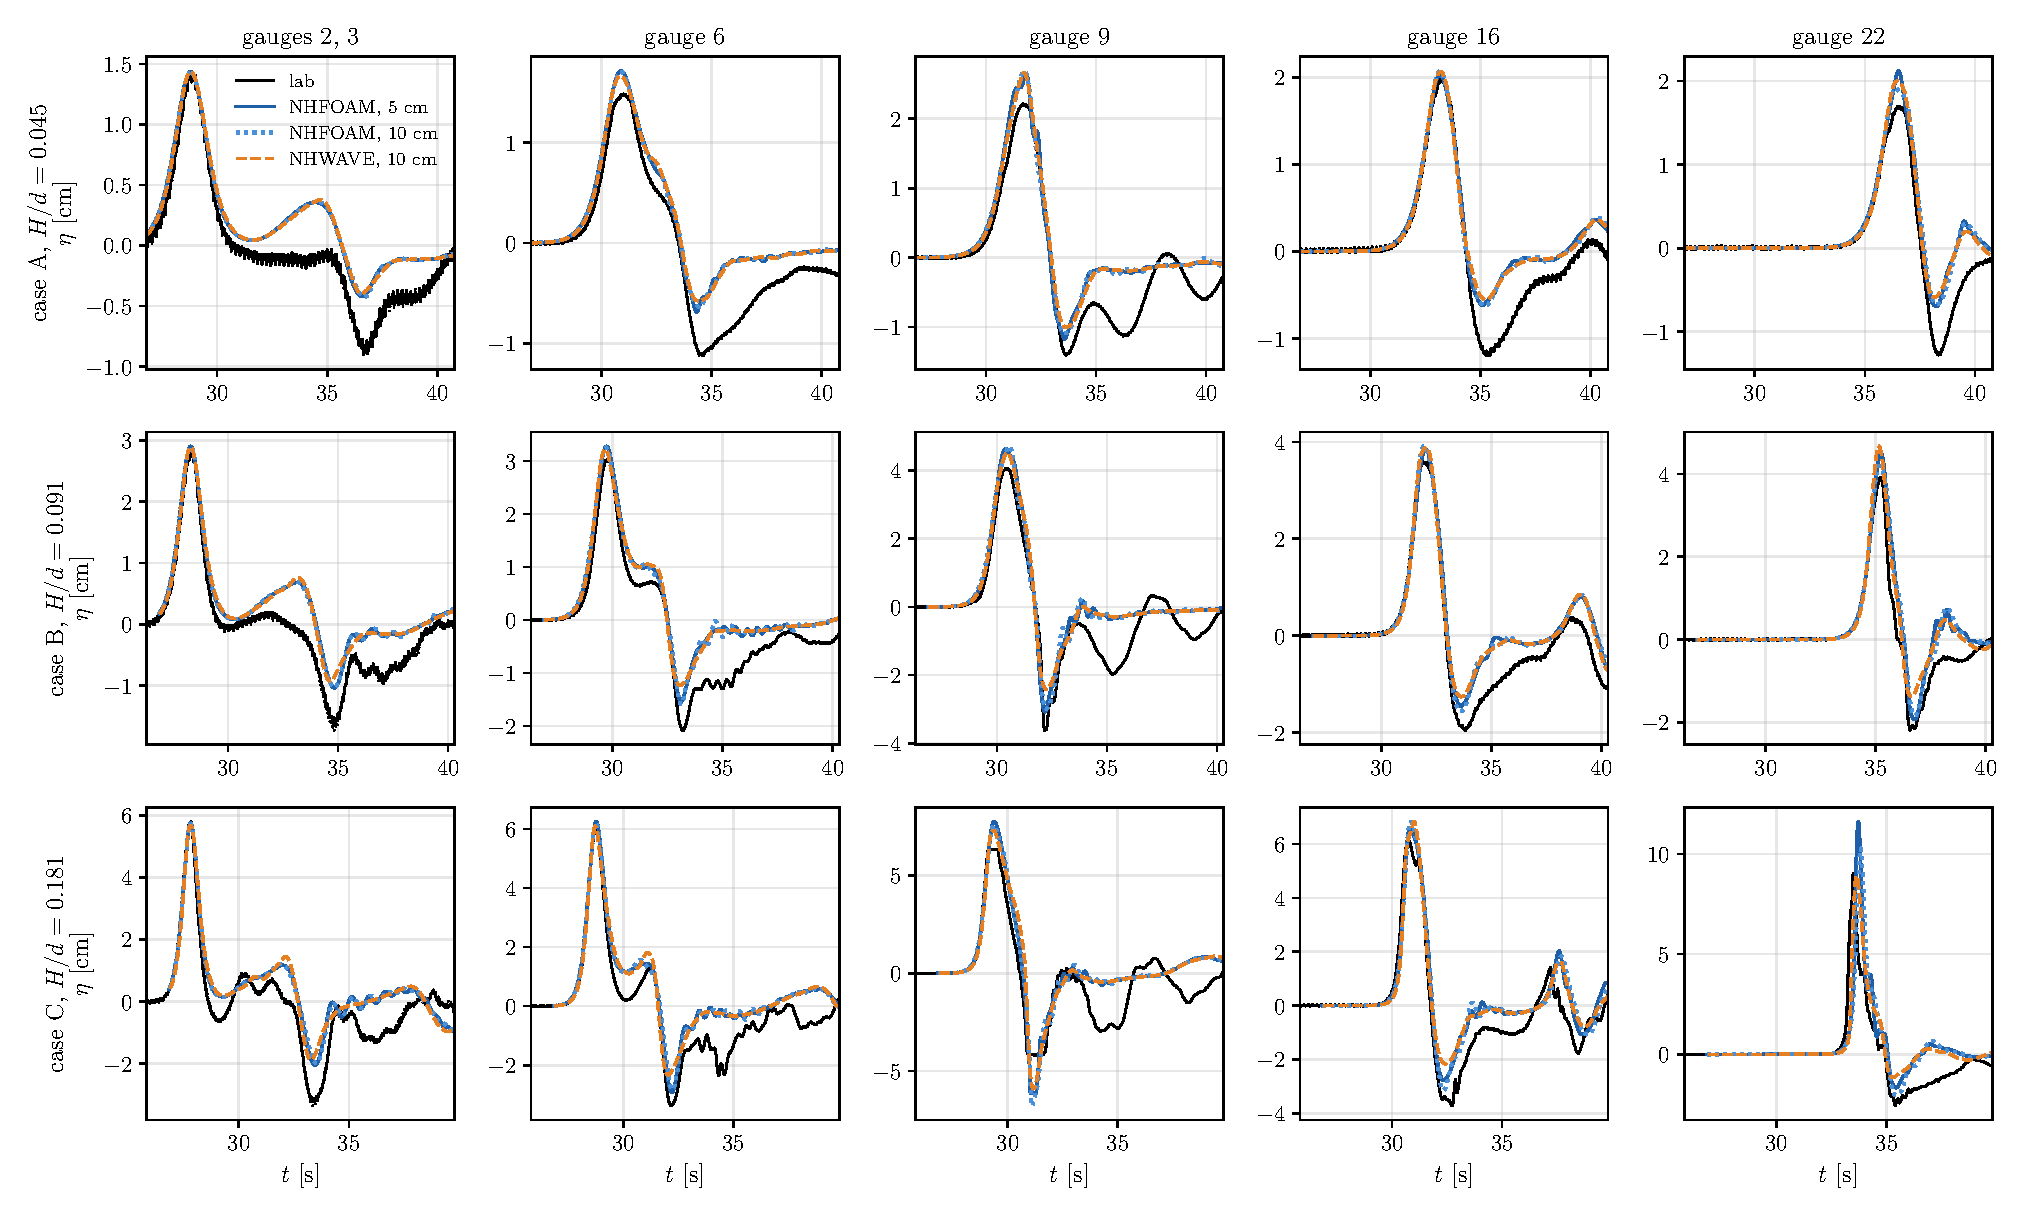
\includegraphics[width=\textwidth]{conical_island_gauges.pdf}
\caption{Solitary waves on a conical island: water level at the gauges against
the measurements of \citet{briggs1995}. The first column shows lab gauges 2
(solid) and 3 (dotted); the model gauge sits at gauge 3, the mirror image of
gauge 2.}
\label{fig:wd-island}
\end{figure}

\begin{figure}[htbp]
\centering
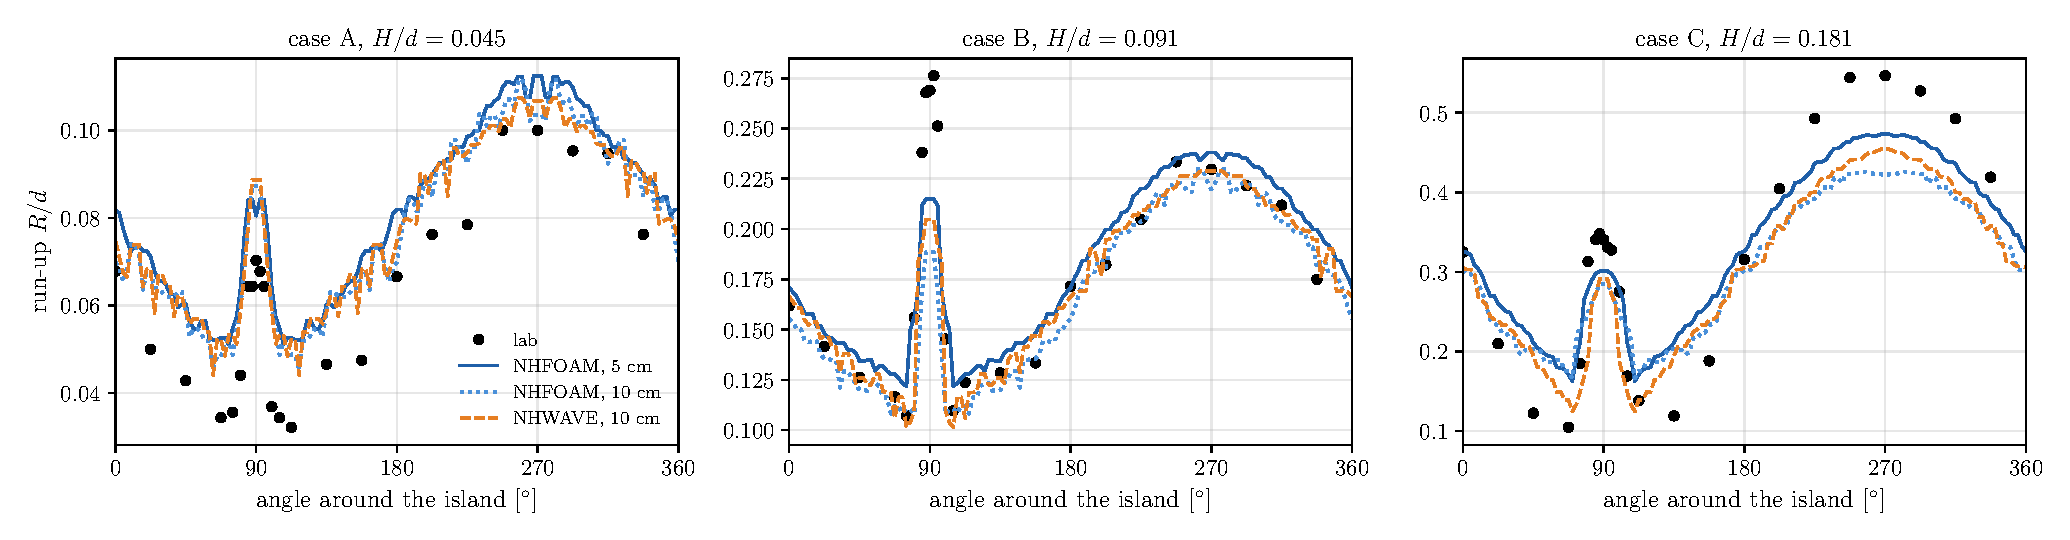
\includegraphics[width=\textwidth]{conical_island_runup.pdf}
\caption{Solitary waves on a conical island: run-up around the island
($0^\circ$ at gauge 16, $90^\circ$ behind the island, $270^\circ$ in front).}
\label{fig:wd-island-runup}
\end{figure}

\subsection{Tsunami run-up in the Monai valley}
\label{sec:wd-monai}

The 1993 Hokkaido Nansei-Oki tsunami ran up 31.7 m at the head of a narrow
valley near Monai, on Okushiri Island. \citet{matsuyama2001} rebuilt the
coast at 1:400 in a 205 m long, 3.5 m wide tank of the Central Research
Institute for Electric Power Industry. The experiment was benchmark 2 of the
2004 workshop on long-wave run-up models \citep{liu2008}; it is benchmark 7
of the NTHMP \citep{synolakis2008} and one of NHWAVE's examples
(\code{Runup\_onto\_a\_complex\_3-D\_beach\_Monai\_Valley}). The benchmark
covers $5.488 \times 3.402$ m with the bed on a 1.4 cm grid: 13.5 cm of water
at $x = 0$, a small island in front of the valley, land up to 12.5 cm above
the still water, and walls on the other three sides. The incident wave is
given at $x = 0$ for 22.5 s, a depression of 2.9 mm followed by a crest of
16.1 mm ($H/d = 0.12$). Gauges 5, 7 and 9 recorded the water level at
$x = 4.521$ m, where the bed file has only 1.2, 0.3 and 0.6 cm of water. In
six repeats the wave ran up 8.0--10.0 cm (mean 9.0 cm) at the head of the
valley, which narrows to 4--6 cm there, and 5.25--6.75 and 5.25--5.75 cm at
two points on its north side.

\NHFOAM\ covers the benchmark domain and takes the incident wave at $x = 0$
as a time series (Section~\ref{sec:ts}) with the active absorption, so that
the boundary lets the reflected waves out, also after 22.5 s, when the
record (tapered to zero over its last 0.5 s) ends. The velocity is uniform
over the depth, $u = c\eta/(d+\eta)$ with $c = \sqrt{g(d+\eta)}$. NHWAVE runs
its example: the domain extended 1.4 m offshore, its internal wavemaker
between $x = -0.14$ and 0 m driven by a Fourier fit of the record (399
components), a 1 m sponge behind it and its $k$--$\varepsilon$ model. Both
models use 4 layers, log-law friction with a roughness of 0.1 mm (NHWAVE's
\code{Zob}) and NHWAVE's 2 mm film; \NHFOAM\ runs its hybrid breaking model.
\NHFOAM\ runs on the benchmark grid (1.4 cm, $392\times243$ columns) and on
the grid coarsened twice (2.8 by 2.79 cm, $196\times122$ columns). On the
benchmark grid NHWAVE takes about 10 s per time step on two cores, about
16 h for the 25 s, so it runs on the coarse grid, with the bed interpolated from the
benchmark nodes and the cell depths the means of the four corners, as
NHWAVE's own depth file has them on the fine grid. On the coarse grid each
model also runs without its breaking treatment (\NHFOAM\ without the
breaking model, NHWAVE without $k$--$\varepsilon$). No run is shifted in
time, and the measured records are shown as given (they read $+2$ to $+5$
mm before the wave arrives). The run-up is the highest ground that a model
floods (the highest bed among the columns that were ever wet), which is how
it was measured: the ground at the three lab points is 8.9, 6.2 and 5.5 cm
high, their mean run-ups. The shorelines at the times of the video frames
of the experiment come from the new \NHFOAM\ option
\code{surfaceSnapshots}, which writes the free surface of every column at
listed times without the full fields, and from NHWAVE's surface output every
0.1 s; the photographs themselves were not compared.

On both grids \NHFOAM's first column follows the record to 0.2 mm rms over
the first 12 s, before the waves reflected from the island and the coast
come back (Fig.~\ref{fig:wd-monai}a). NHWAVE's wavemaker keeps time with the
record too (lag 0.001 s), with a deeper depression (3.5 against 2.9 mm) and
a 2\% lower crest (0.6 mm rms). After 12 s both boundaries let the same
reflected waves out.

The depression dries all three gauge columns in both models (the flat parts
of Fig.~\ref{fig:wd-monai} at 12--15 s), while the measured records stay wet:
gauge 7 reads 0.6 cm below the still water at 14 s, where the bed file puts
the bed at $-0.27$ cm, so the gauges stood in deeper water than the file has
at their positions. The bore then floods the dried bed. \NHFOAM's arrives
0.03--0.39 s after the measured one on both grids, NHWAVE's 0.30--0.40 s,
about the 0.4 s by which NHWAVE's example shifts its results
(Table~\ref{tab:wd-monai}). Behind the bore both models follow the measured
records, with rms differences of 0.5--0.6 cm. \NHFOAM's short crests at
17--17.6 s are 13--18\% higher than the measured ones on the coarse grid and
21--29\% on the benchmark grid; NHWAVE's smoother crests are 1--5\% lower.

On the coarse grid the two models flood almost the same columns (0.64 and
0.63 m$^2$ of land; \NHFOAM\ floods every column that NHWAVE floods) and run
up 6.6 cm at the head of the valley, 27\% below the measured mean, and
4.3 cm at the two points to the north, 23--29\% low
(Fig.~\ref{fig:wd-monai-runup}, Table~\ref{tab:wd-monai-runup}): the head of
the valley is only one or two coarse cells wide. On the benchmark grid
\NHFOAM\ runs up 7.4 cm at the head (17\% low, below the lowest of the six
repeats), 5.4 cm at the first point to the north (within the measured
5.25--6.75 cm) and 4.4 cm at the second (21\% low). The shorelines of the two
grids agree at the times of the video frames (Fig.~\ref{fig:wd-monai-frames});
NHWAVE's lags behind \NHFOAM's while the water climbs the valley (by 0.27 m
at 15.3 s and 0.17 m at 15.8 s) and has caught up by 16.8 s.

Without its breaking model \NHFOAM's crest at gauge 5 is 9\% higher (4.70
against 4.31 cm), and the bore, the rms differences and the run-up do not
change. Without $k$--$\varepsilon$ NHWAVE's crests are 1--3\% higher and its
bore arrives 0.02 s earlier, with the same run-up. Neither closure explains
the differences between the models: with or without them NHWAVE's bore
reaches gauges 7 and 9 0.3 s after \NHFOAM's, and \NHFOAM's short crests
stay 11--29\% above NHWAVE's. The difference lies in how the bore runs over
the dried bed: NHWAVE's shoreline also lags behind \NHFOAM's while the water
climbs the valley.
On the coarse grid \NHFOAM\ took 35 min and NHWAVE 2.0 h on two cores
(1.7 h without $k$--$\varepsilon$); \NHFOAM\ took 6.2 h on the benchmark
grid.

\begin{table}[htbp]
\centering
\caption{Monai valley, gauges over 13--23 s: highest crest against the
measured one, arrival of the bore ($\eta$ rising through 0.5 cm) against the
measured arrival, and rms difference.}
\label{tab:wd-monai}
\footnotesize
\setlength{\tabcolsep}{4pt}
\begin{tabular}{lrrrrrrrrr}
\toprule
run & \multicolumn{3}{c}{crest} & \multicolumn{3}{c}{bore arrival [s]} & \multicolumn{3}{c}{rms [cm]} \\
\cmidrule(lr){2-4}\cmidrule(lr){5-7}\cmidrule(lr){8-10}
 & g5 & g7 & g9 & g5 & g7 & g9 & g5 & g7 & g9 \\
\midrule
lab & 3.70 cm & 3.92 cm & 4.54 cm & 14.59 & 14.81 & 14.95 & & & \\
\NHFOAM, 1.4 cm & +21\% & +24\% & +29\% & +0.39 & +0.11 & +0.03 & 0.58 & 0.52 & 0.58 \\
\NHFOAM, 2.8 cm & +16\% & +13\% & +18\% & +0.36 & +0.12 & +0.03 & 0.57 & 0.53 & 0.59 \\
NHWAVE, 2.8 cm & $-3$\% & $-1$\% & $-5$\% & +0.34 & +0.40 & +0.30 & 0.62 & 0.53 & 0.58 \\
\NHFOAM, 2.8 cm, no breaking & +27\% & +14\% & +20\% & +0.36 & +0.11 & +0.03 & 0.58 & 0.53 & 0.60 \\
NHWAVE, 2.8 cm, no $k$--$\varepsilon$ & $-1$\% & +2\% & $-3$\% & +0.32 & +0.38 & +0.28 & 0.62 & 0.52 & 0.60 \\
\bottomrule
\end{tabular}
\end{table}

\begin{table}[htbp]
\centering
\caption{Monai valley: run-up at the measured points, the head of the
valley (5.158, 1.880) m and two points on its north side, N1 (5.030, 2.206)
m and N2 (4.998, 2.320) m (lab: the six repeats), the
highest flooded ground in the valley ($1.75 < y < 2.05$ m), the flooded land
and the run time on two cores.}
\label{tab:wd-monai-runup}
\footnotesize
\setlength{\tabcolsep}{4pt}
\begin{tabular}{lrrrrrr}
\toprule
run & \multicolumn{3}{c}{run-up at the lab points [cm]} & highest in the & flooded & time \\
\cmidrule(lr){2-4}
 & head & N1 & N2 & valley [cm] & land [m$^2$] & \\
\midrule
lab, range & 8.0--10.0 & 5.25--6.75 & 5.25--5.75 & & & \\
lab, mean & 9.0 & 6.0 & 5.6 & & & \\
\NHFOAM, 1.4 cm & 7.4 & 5.4 & 4.4 & 7.5 & 0.65 & 6.2 h \\
\NHFOAM, 2.8 cm & 6.6 & 4.3 & 4.3 & 6.9 & 0.64 & 35 min \\
NHWAVE, 2.8 cm & 6.6 & 4.3 & 4.3 & 6.6 & 0.63 & 2.0 h \\
\NHFOAM, 2.8 cm, no breaking & 6.6 & 4.3 & 4.3 & 6.9 & 0.64 & 35 min \\
NHWAVE, 2.8 cm, no $k$--$\varepsilon$ & 6.6 & 4.3 & 4.3 & 6.6 & 0.64 & 1.7 h \\
\bottomrule
\end{tabular}
\end{table}

\begin{figure}[htbp]
\centering
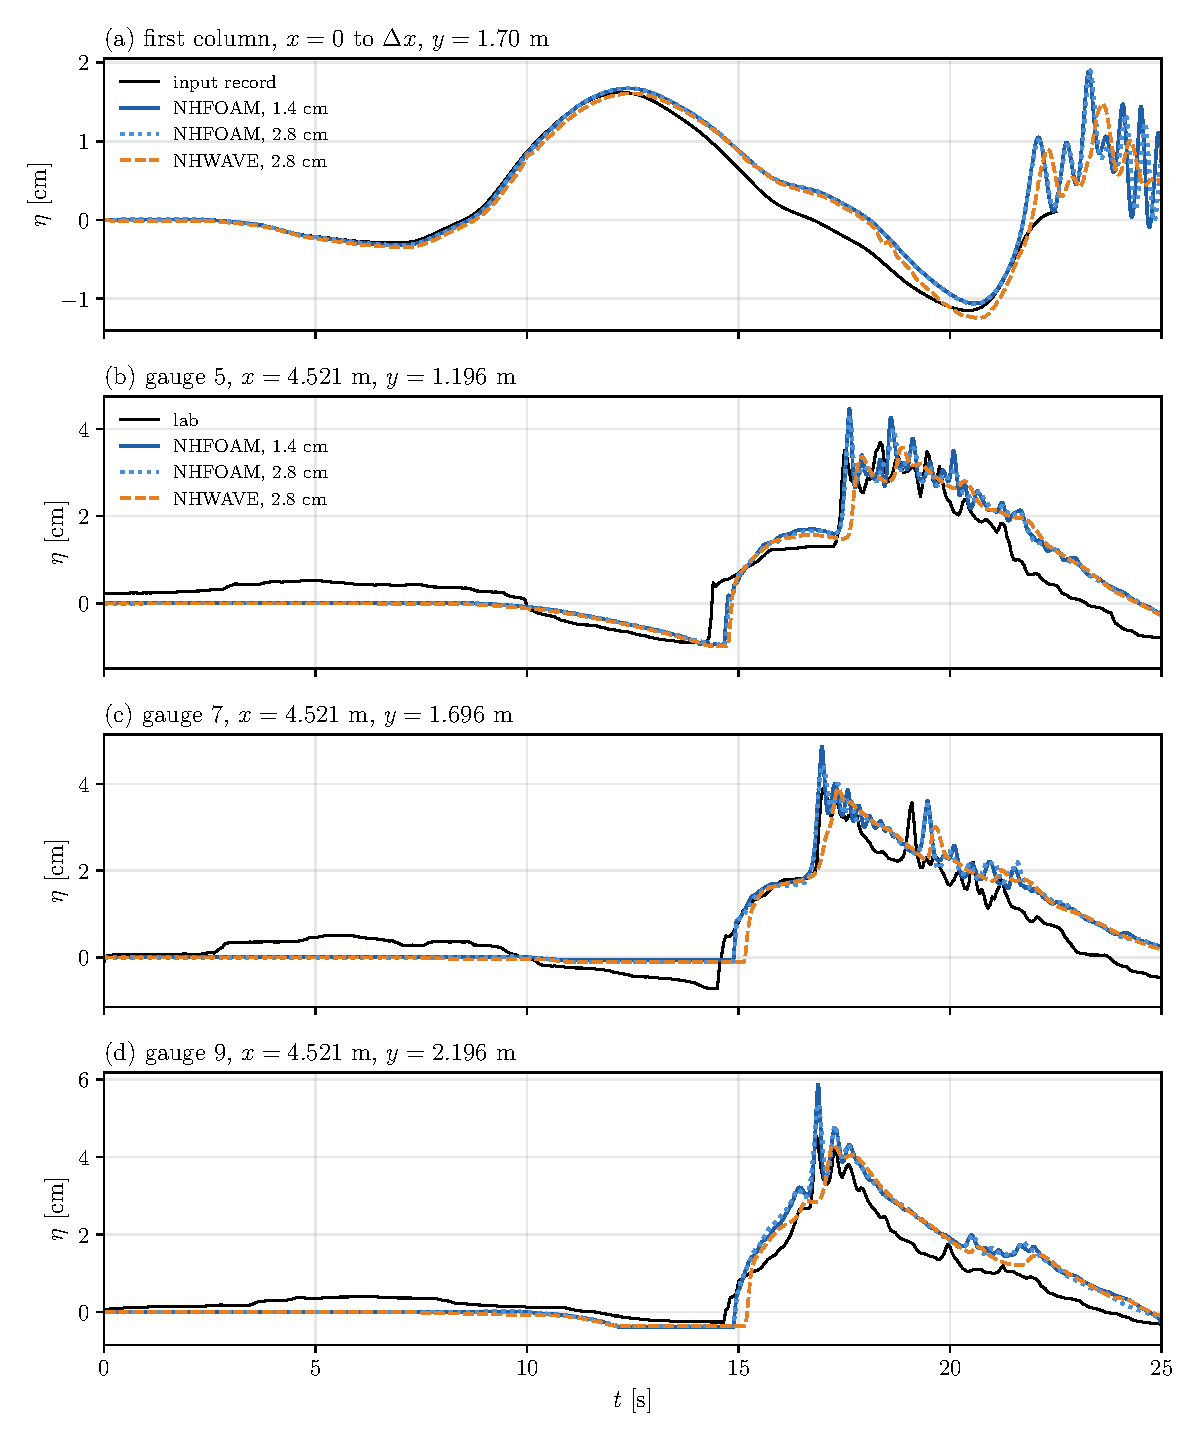
\includegraphics[width=0.85\textwidth]{monai_valley_gauges.pdf}
\caption{Monai valley: (a) the surface of the first column ($y = 1.70$ m)
against the input record; (b--d) water level at gauges 5, 7 and 9 against
the measurements of \citet{matsuyama2001}.}
\label{fig:wd-monai}
\end{figure}

\begin{figure}[htbp]
\centering
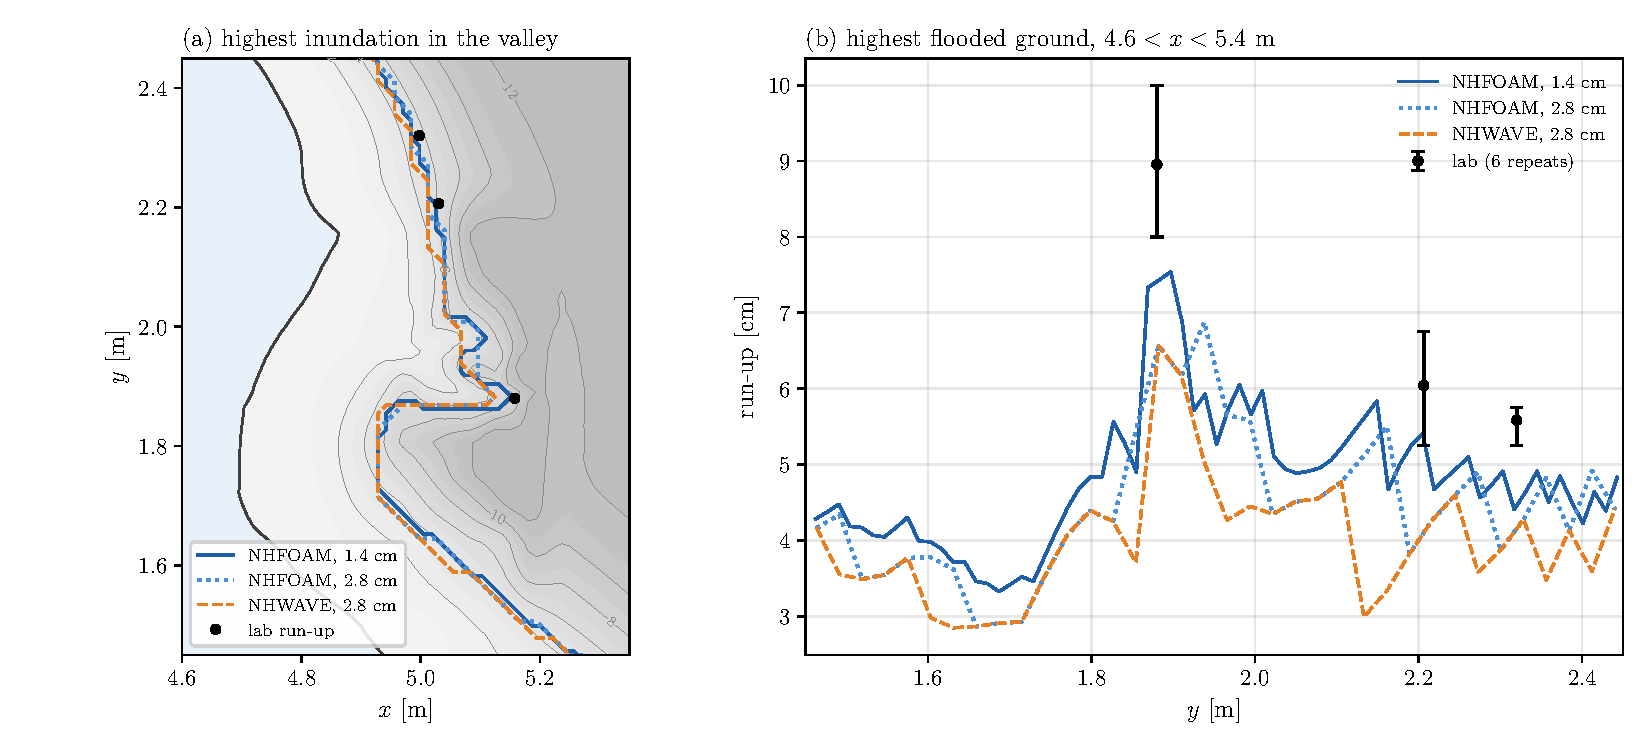
\includegraphics[width=\textwidth]{monai_valley_runup.pdf}
\caption{Monai valley: (a) the edge of the flooded area around the valley
(ground shaded by its height, contours every 2 cm, the still-water shoreline
thick) and the points of the measured run-up; (b) the highest flooded ground
along the valley ($4.6 < x < 5.4$ m) against the measured run-up (range of
the six repeats).}
\label{fig:wd-monai-runup}
\end{figure}

\begin{figure}[htbp]
\centering
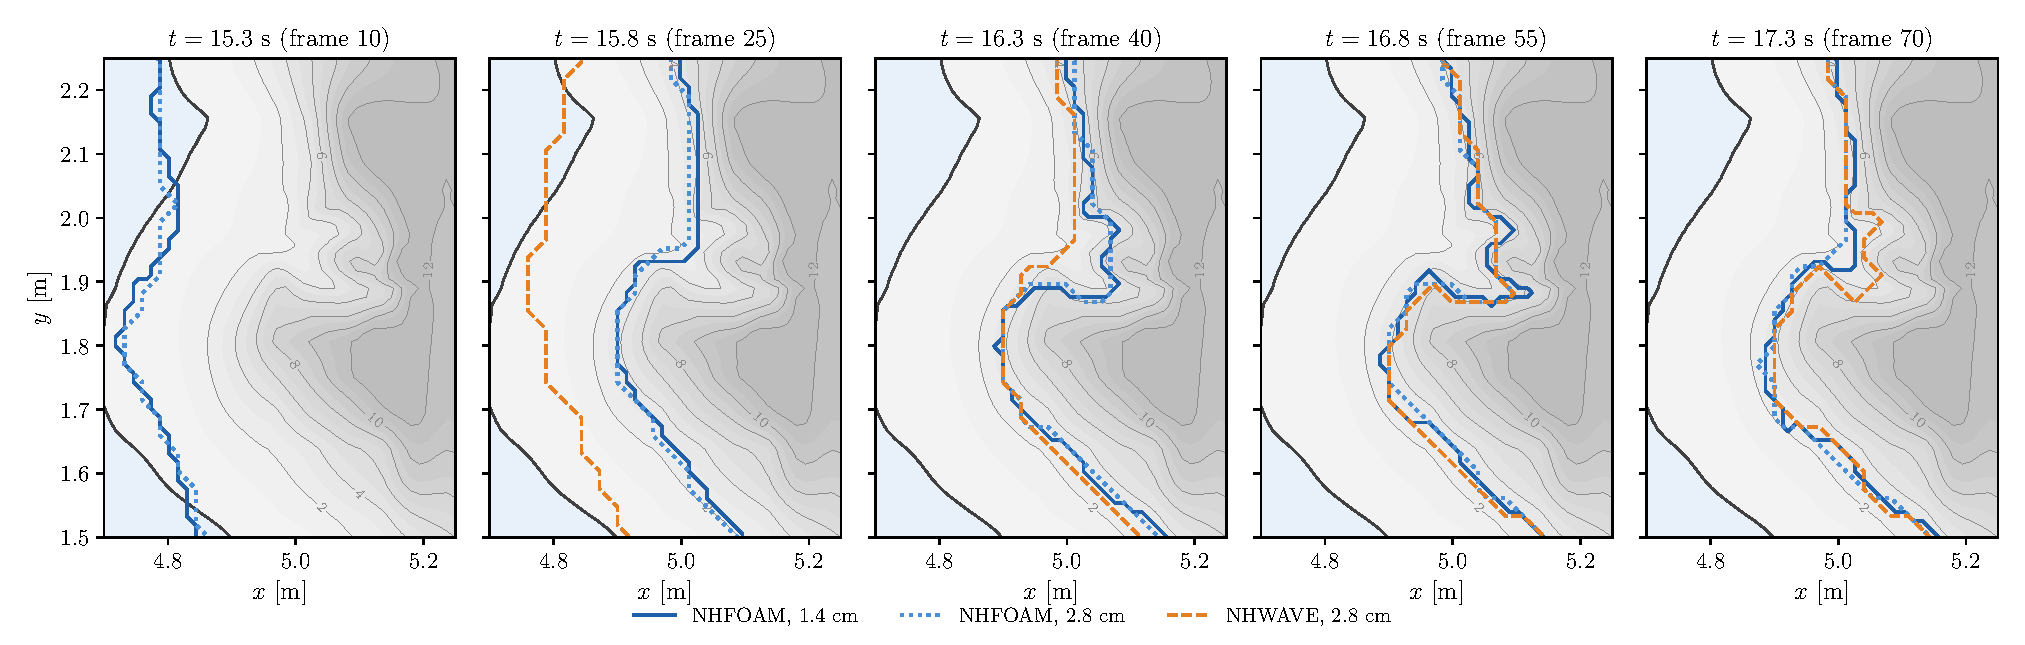
\includegraphics[width=\textwidth]{monai_valley_frames.pdf}
\caption{Monai valley: shorelines at the times of frames 10--70 of the video
of the experiment ($t = 15.3$--17.3 s, as the benchmark gives them). At
15.3 s NHWAVE's shoreline still lies seaward of the frame ($x < 4.7$ m).}
\label{fig:wd-monai-frames}
\end{figure}

\subsection{The Monai valley on a mesh refined around the valley}
\label{sec:wd-monai-ref}

On the uniform grids the run-up at the head of the valley stays 17\%
(1.4 cm) to 27\% (2.8 cm) below the measured mean. The valley narrows to
4--6 cm there, and a uniform grid pays for the resolution of the valley over
the whole basin. NHWAVE has no other choice; \NHFOAM\ takes any mesh that is
made of columns (Section~\ref{sec:unstr}). Here the basin is meshed with
gmsh quadrilaterals whose size follows the depth, $5.6\sqrt{h/d}$ cm down to
2.8 cm in the shallow water and on the land that the wave can reach, with
smaller cells in a box of $0.45 \times 0.7$ m around the valley and the three
lab points and, as an option, on the shelf in front of it ($1.3 \times 1.5$
m, with the gauges), extruded into 4 layers (Fig.~\ref{fig:wd-monai-ref}a).
Everything else is the set-up of Section~\ref{sec:wd-monai}. The time step
follows the Courant number (at most 1) below 8 ms, the step of the uniform
2.8 cm grid, so the small cells cost time steps only while water moves
through them: the smallest step is 2--4 ms and the runs take 3150--3530
steps. The bed is still the bilinear interpolation of the 1.4 cm benchmark
data, so cells below 1.4 cm add numerical resolution and no detail of the
bed.

\begin{table}[htbp]
\centering
\caption{Monai valley on uniform grids and on meshes refined around the
valley: run-up at the head of the valley and at the two points to its north
(N1, N2), the highest flooded ground in the valley and the run time on two
cores.}
\label{tab:wd-monai-ref}
\footnotesize
\setlength{\tabcolsep}{4pt}
\begin{tabular}{lrrrrrrr}
\toprule
mesh & columns & steps & \multicolumn{3}{c}{run-up [cm]} & valley & time \\
\cmidrule(lr){4-6}
 & & & head & N1 & N2 & [cm] & \\
\midrule
lab, range & & & 8.0--10.0 & 5.25--6.75 & 5.25--5.75 & & \\
lab, mean & & & 9.0 & 6.0 & 5.6 & & \\
uniform 2.8 cm & 23\,912 & 3125 & 6.6 & 4.3 & 4.3 & 6.9 & 35 min \\
uniform 1.4 cm & 95\,256 & 6250 & 7.4 & 5.4 & 4.4 & 7.5 & 6.2 h \\
valley 1.4 cm & 16\,883 & 3150 & 7.0 & 4.7 & 4.3 & 7.4 & 16 min \\
shelf and valley 1.4 cm & 22\,962 & 3163 & 7.1 & 5.8 & 4.7 & 7.8 & 22 min \\
valley 0.7 cm & 22\,455 & 3264 & 8.1 & 5.7 & 4.9 & 8.3 & 22 min \\
shelf 1.4 cm, valley 0.7 cm & 28\,279 & 3282 & 8.1 & 5.6 & 5.1 & 8.2 & 28 min \\
valley 0.7 cm, head 0.35 cm & 24\,897 & 3528 & 8.5 & 5.8 & 5.1 & 8.5 & 27 min \\
valley 0.7 cm, triangles & 52\,929 & 3891 & 8.3 & 5.6 & 5.3 & 8.3 & 64 min \\
\bottomrule
\end{tabular}
\end{table}

The resolution of the valley decides the run-up
(Table~\ref{tab:wd-monai-ref}, Fig.~\ref{fig:wd-monai-ref}). With 0.7 cm
cells in the valley the run-up at the head is 8.1 cm, inside the measured
8.0--10.0 cm, and 5.7 cm at N1 (measured 5.25--6.75 cm); N2 stays 12\% below
the measured mean. That mesh has fewer columns than the uniform 2.8 cm grid
and ran in 22 min, against 6.2 h for the uniform 1.4 cm grid, which gives
7.4 cm: a quarter of the columns and, with the adaptive step that the
uniform runs did not use, half the time steps. With 1.4 cm on the shelf and
in the valley the refined mesh gives the run-up of the uniform 1.4 cm grid
within 0.3 cm at the three points and its crests at the gauges ($+21$, $+17$
and $+25\%$ against $+21$, $+24$ and $+29\%$). Meshes of the same nominal
resolution differ by 0.1--0.3 cm at a point, as the run-up is read from the
bed height of single columns.

The shelf matters for the gauges and not for the head of the valley: with
0.7 cm in the valley, the shelf at 1.4 cm instead of 2.8 cm leaves the
run-up at the head at 8.1 cm, while on every refined mesh the bore reaches
the gauges within 0.04 s of the uniform grid with the same resolution on the
shelf, with the same rms differences (0.50--0.60 cm). The run-up at the head
is not yet converged: with 0.35 cm cells there ($0.32 \times 0.22$ m) it
rises again, to 8.5 cm, so that from 2.8 to 0.35 cm it goes 6.6, 7.0--7.4,
8.1 and 8.5 cm (lab mean 9.0 cm).
The same mesh in triangles (edges of the same length, so 2.4 times the
columns) runs up 8.3, 5.6 and 5.3 cm, within 0.4 cm of the
quadrilaterals' 8.1, 5.7 and 4.9 cm, with the same gauges, at three
times the cost; the 8\% lower run-up of the triangulated strip of
Section~\ref{sec:unstr} does not show here.
The film is not the limit: on the uniform 2.8 cm grid, films of 2, 1 and
0.5 mm give the same run-up at all three points and crests within 5\% of
each other; with the thinner films the bore reaches
gauge 5 0.15 s earlier and gauge 9 0.07--0.11 s later.

\begin{figure}[htbp]
\centering
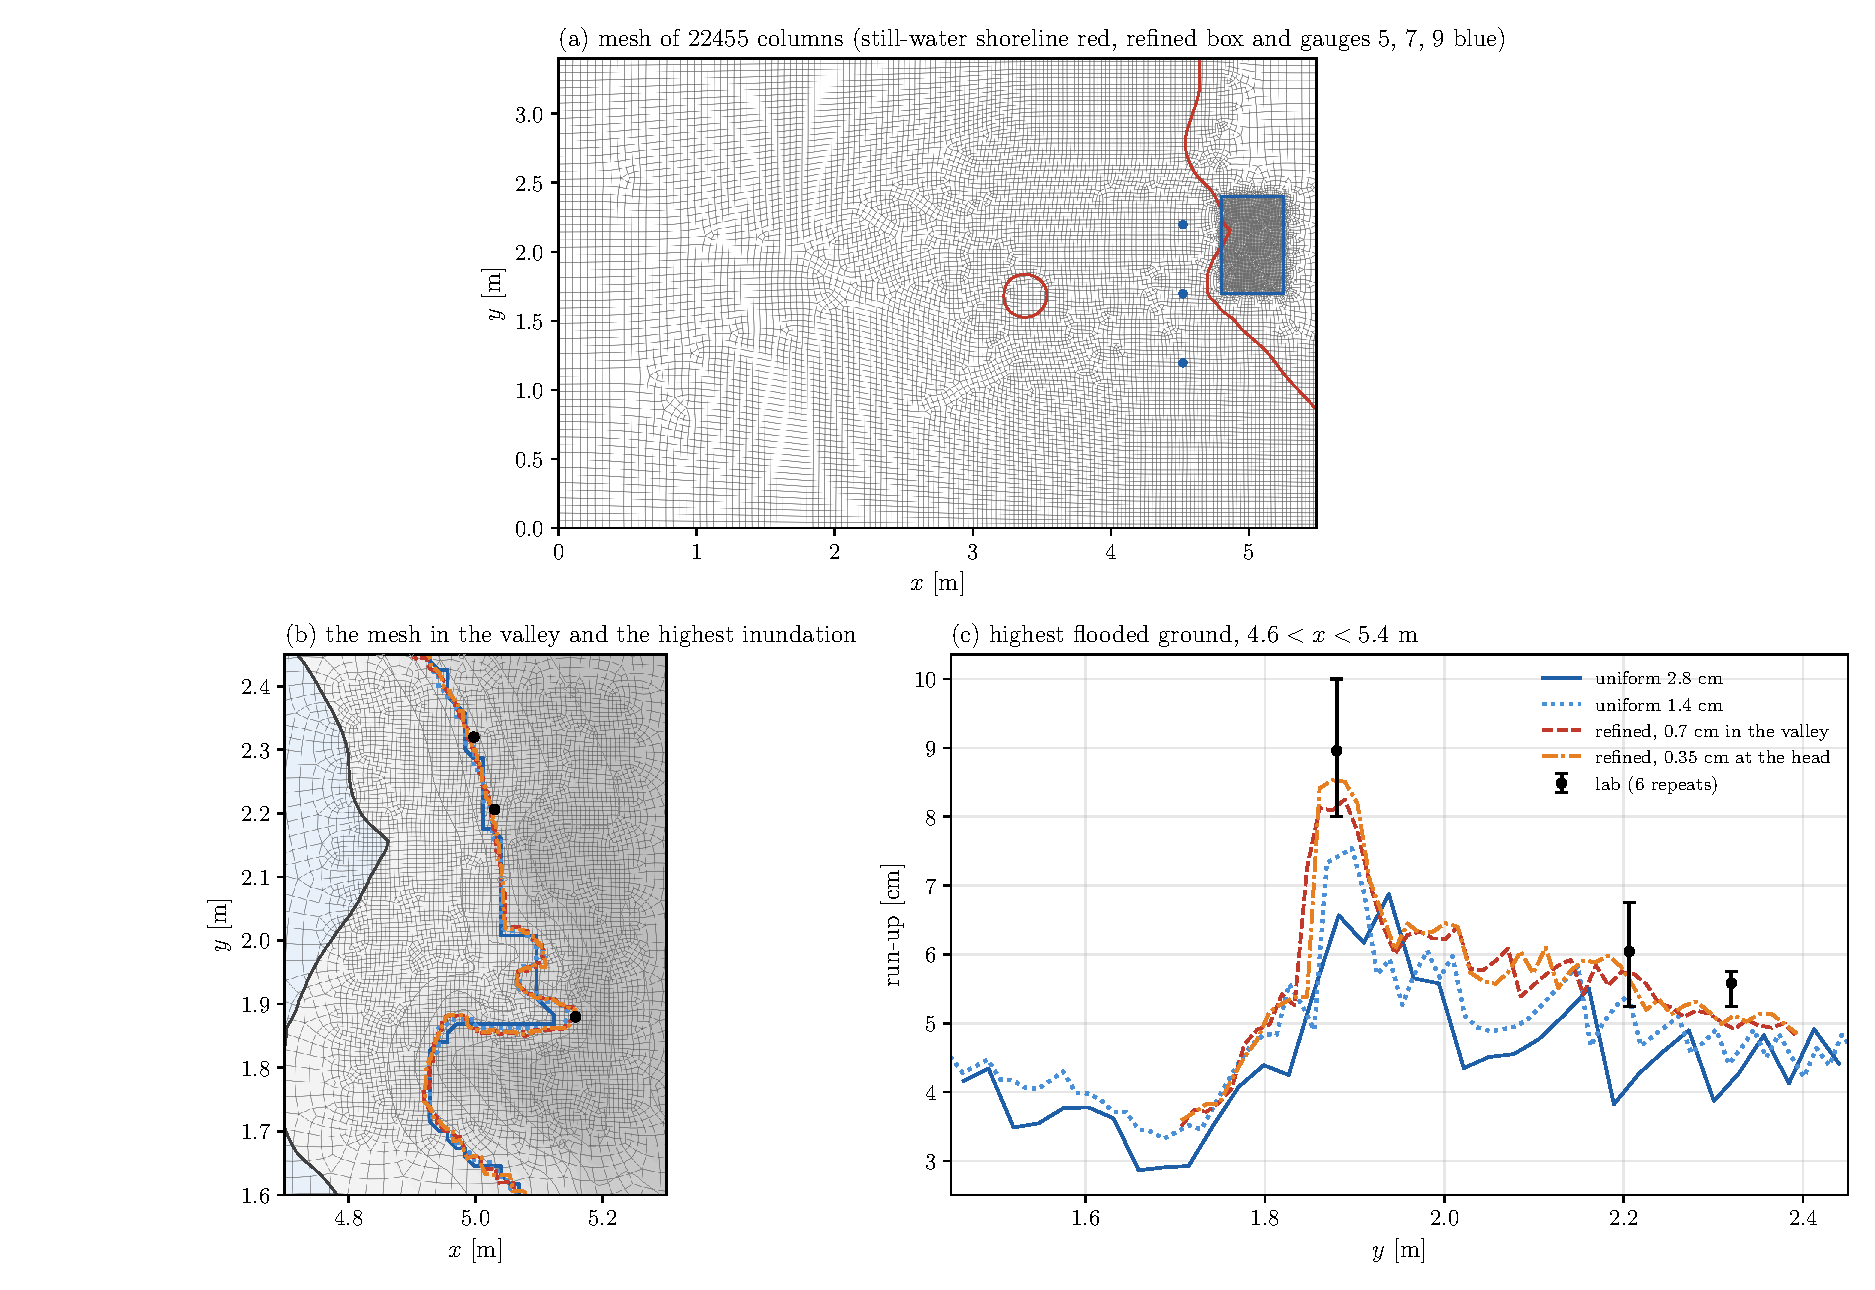
\includegraphics[width=\textwidth]{monai_valley_refined.pdf}
\caption{Monai valley on a mesh refined around the valley: (a) the mesh with
0.7 cm cells in the valley; (b) the mesh in the valley, the edge of the
flooded area and the points of the measured run-up; (c) the highest flooded
ground along the valley against the measured run-up (range of the six
repeats).}
\label{fig:wd-monai-ref}
\end{figure}

\subsection{Spilling breakers on a 1:35 beach}
\label{sec:wd-tk}

\citet{ting1994} measured spilling breakers of $H = 0.125$ m and $T = 2$ s from
$h = 0.4$ m on a 1:35 beach. Here $x$ is measured from the toe of the slope,
which reproduces the measured breaking point; the still-water shoreline is
at $x = 14$ m. \NHFOAM\ makes stream-function waves in a 3.8 m relaxation zone,
2.2 m ahead of the toe, and runs onto dry land up to $x = 17$ m: 10 layers,
$\Delta x = 2.5$ cm, $\Delta t = 5$ ms, a 5 mm film, $C_d = 0.006$, the
hydrostatic front approximation with $\alpha = 0.6$ and $\beta = 0.3$. NHWAVE
runs its example \code{tingkirby}, with 20 layers, the $k$--$\epsilon$ model, a
cnoidal wave at the boundary and a 2 cm film. Its bed has the toe 5.6 m from
the wavemaker, so its $x$ is shifted by 5.6 m. Both runs last 60 s, and the
statistics use the last 10 periods (Fig.~\ref{fig:wd-tk},
Table~\ref{tab:wd-tk}).

\begin{figure}[ht]
\centering
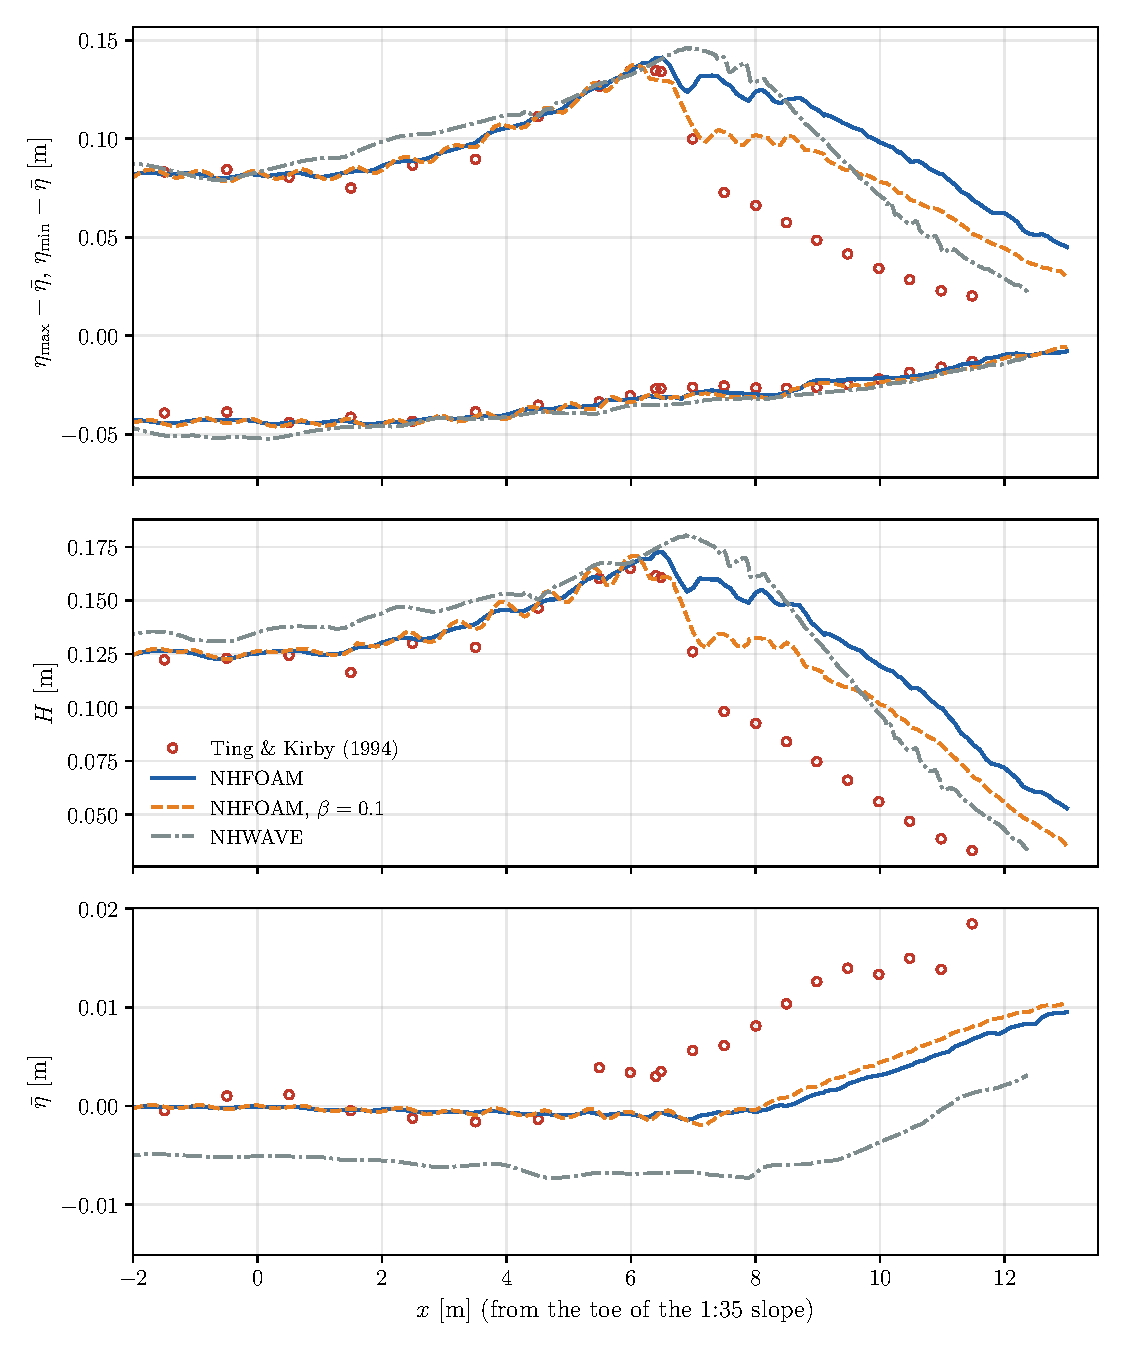
\includegraphics[width=0.9\textwidth]{tk_spilling.pdf}
\caption{Spilling breakers \citep{ting1994}: crest and trough relative to the
mean level, wave height and mean water level.}
\label{fig:wd-tk}
\end{figure}

\begin{table}[ht]
\centering
\caption{Spilling breakers: wave height and mean water level (cm).}
\label{tab:wd-tk}
\small
\begin{tabular}{lcccc}
\toprule
 & lab & \NHFOAM & \NHFOAM, $\beta = 0.1$ & NHWAVE \\
\midrule
$H$ at $x = -0.5$ m & 12.3 & 12.3 & 12.3 & 13.1 \\
largest $H$, at $x$ & 16.5, 6.0 m & 17.3, 6.5 m & 17.1, 6.1 m & 18.0, 6.9 m \\
$H$ at $x = 8$ m & 9.3 & 15.4 & 13.3 & 16.1 \\
$H$ at $x = 11$ m & 3.9 & 10.0 & 8.3 & 6.4 \\
rms error of $H$, $x < 6$ m & & 0.5 & 0.6 & 1.4 \\
mean error of $H$, $x > 7$ m & & $+6.1$ & $+4.2$ & $+4.8$ \\
mean level at $x = 11$ m & 1.4 & 0.5 & 0.7 & 0.0 \\
\bottomrule
\end{tabular}
\end{table}

Up to breaking \NHFOAM\ follows the measurements: the incident height is
right, the rms error before $x = 6$ m is 0.5 cm, and the waves break 0.5 m
later than in the flume and 0.8 cm higher. NHWAVE's waves are 0.8 cm too high
from the start and break 0.9 m late. Inside the surf zone both models lose too
little energy. The heights decay more slowly than the measured ones, and the
mean level rises too late and too little. At $x = 8$ m the waves are 6 cm
(\NHFOAM) and 7 cm (NHWAVE) higher than the measured 9.3 cm, and near the
shoreline NHWAVE's $k$--$\epsilon$ dissipation brings its heights closer. In
\NHFOAM\ the waves of the inner surf zone are sawtooth bores with $H/h$ near 1,
of which only the one or two columns at the front are flagged as breaking.
Two sensitivity runs locate the problem. Keeping columns breaking down to
$\beta = 0.1$ flags 10--12 columns, moves the breaking point to $x = 6.1$ m
and cuts the surf-zone error by a third. Switching $q$ off in all columns
shallower than 0.23 m (\code{hydrostaticDepth}) leaves +2.8 cm, and three
layers instead of ten change nothing (+6.3 cm). The core scheme captures
hydrostatic bores: a dam break onto a 2 cm bed gives the height and speed of
Stoker's bore within about 1\%. What is missing is dissipation where the
non-hydrostatic pressure acts behind the flagged front; Section~\ref{sec:brk}
adds it.
The upwind face depth did not change this. The test confirms the limitation
found with the breakers of \citet{hansen1979} (Section~\ref{sec:breaking}),
now with a full beach, set-up and NHWAVE alongside.
